\begin{footnotesize}
\newcommand{\participK}[2]{
\begin{scope}[shift={(#1)}]
\draw [draw,fill=lightgray] (0pt,10pt) circle (5pt);
\draw [draw,fill=lightgray] (10pt,0pt) arc (0:180:10pt and 5pt);
\fill [lightgray] (-10pt,-10pt) rectangle (10pt,0pt);
\draw [draw] (10pt,0pt) -- (10pt,-10pt);
\draw [draw] (-10pt,0pt) -- (-10pt,-10pt);
\draw [draw] (5pt,-1pt) -- (5pt,-10pt);
\draw [draw] (-5pt,-1pt) -- (-5pt,-10pt);
\draw [anchor=center] (0pt,-2.5pt) node {#2};
\end{scope}
}
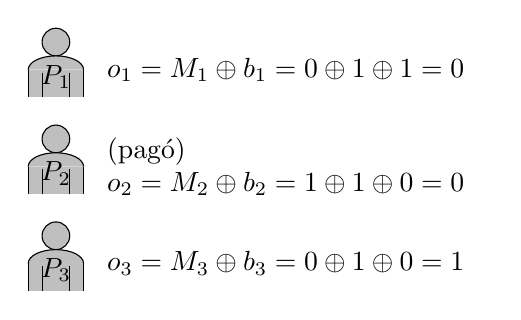
\begin{tikzpicture}

\begin{scope}
\path (0em,7em) coordinate (Q1);
\path (0em,3.5em) coordinate (Q2);
\path (0em,0em) coordinate (Q3);

\node [rectangle, right of=Q1, anchor=west, node distance=1.5em] {$o_1 = M_1 \oplus b_1 = 0 \oplus 1 \oplus 1 = 0$};
\node [rectangle, right of=Q2, anchor=west, node distance=1.5em, text width=136pt] {(pagó)\\$o_2= M_2 \oplus b_2 = 1 \oplus 1 \oplus 0 = 0$};
\node [rectangle, right of=Q3, anchor=west, node distance=1.5em] {$o_3= M_3 \oplus b_3 = 0 \oplus 1 \oplus 0 = 1$};

\participK{Q1}{$P_1$};
\participK{Q2}{$P_2$};
\participK{Q3}{$P_3$};
\end{scope}

\end{tikzpicture}
\end{footnotesize}
